\section{Comparison with Alternative Approaches}
\label{sec:comparison}

The evaluation in \S\ref{sec:evaluation} establishes that \eps fires on
the prompts it is designed to catch. What it does not establish is
whether \eps is the right signal relative to alternatives that read the
same raw logprob data, or to alternatives that use the same underlying
model via a different protocol. This section provides that comparison
along two axes: signal structure (what each method measures) and
empirical performance on the same four-model benchmark.

\subsection{Signal taxonomy}
\label{subsec:signal-taxonomy}

Three fundamentally different uncertainty signals are in play.
\textbf{Intra-generational token-level entropy} (\eps; AdaDec) reads the
top-$k$ distribution at each decoding step. \textbf{Sequence-level
aggregate probability} (\papg; the Spiess et al.~\cite{spiess2025calibration}
signal) averages log-probabilities over all generated tokens to produce
a single scalar per function. \textbf{Inter-generational behavioural
diversity} (multi-sample methods, UQLM~\cite{uqlm2024}) runs the model
multiple times at nonzero temperature and measures output-level
agreement.

These are not three implementations of the same idea. The first two
happen to read the same raw logprob data at the same $1\times$ API cost,
but aggregate it differently: \eps localizes to a single high-entropy
token after syntactic filtering, while \papg smooths over the entire
sequence. The third requires multiple model calls and measures a
fundamentally different quantity: it cannot observe internal
distributions at all, only the outputs those distributions produce.

\subsection{\papg: competitive on rate, silent on location}
\label{subsec:papg-comp}

We compute \papg directly from the \texttt{mean\_logprob} fields in the
same calibration runs used to produce Table~\ref{tab:calibration}:
$\papg = \exp(\mathrm{mean\_logprob})$, with higher values indicating
higher confidence. For a fair comparison, we choose the \papg decision
threshold on each model so that the resulting LOW false-positive rate
matches \eps's rate on that model; we then report the HIGH detection
rate achieved at that operating point.

\begin{table}[h]
\centering
\small
\begin{tabular}{lrrrr}
\toprule
 & \multicolumn{2}{c}{\eps (\textsc{flagged+})} & \multicolumn{2}{c}{\papg (matched FP)} \\
\cmidrule(lr){2-3}\cmidrule(lr){4-5}
Model & HIGH det. & LOW FP & HIGH det. & LOW FP \\
\midrule
GPT-4o       & $85\%$ (17/20) & $50\%$ & $85\%$ (17/20) & $50\%$ \\
GPT-4o-mini  & $70\%$ (14/20) & $60\%$ & $75\%$ (15/20) & $10\%$ \\
GPT-4-turbo  & $70\%$ (14/20) & $60\%$ & $90\%$ (18/20) & $40\%$ \\
DeepSeek V3  & $85\%$ (17/20) & $70\%$ & $65\%$ (13/20) & $10\%$ \\
\bottomrule
\end{tabular}
\caption{\eps vs.\ \papg across four models. \papg ties \eps on GPT-4o
and outperforms \eps on GPT-4o-mini and GPT-4-turbo on raw HIGH
detection; on DeepSeek V3, \eps is higher ($85\%$ vs.\ $65\%$). At the
same $1\times$ API cost, the raw-detection picture favours neither
signal uniformly.}
\label{tab:papg}
\end{table}

Two facts account for the pattern. First, \papg averages over all
tokens, so long stretches of confident boilerplate dilute a single high-%
entropy decision; \eps max-pools after AST filtering, so an API-selector
token at $\eps = 0.73$ dominates the function-level score regardless of
length. On prompts where the uncertain decision is a small fraction of
the generated tokens, \papg's low denominator on the long confident
portion can nevertheless yield a probability low enough to fire, because
even the confident tokens for some OpenAI model families carry
non-trivial probability mass on alternates. Second, on naming-heavy LOW
prompts, \papg's averaging suppresses the cosmetic variation that
drives \eps's false-positive rate above $50\%$, which is why some OpenAI
models show higher \papg LOW specificity. On DeepSeek V3, where
vocabulary is larger and per-token entropy is higher on cosmetic tokens,
the averaging does not save \papg and \eps is the better signal.

The key distinguishing property of \eps is not higher detection but
\emph{localization}. \papg produces one scalar per function; \eps
identifies that ``\texttt{stripe.Charge} $P=0.52$ vs.\
\texttt{stripe.PaymentIntent} $P=0.47$ at the method-selector token''
is the uncertain decision. The stage-2 reviewer uses this attribution
to target its analysis: when the high-\eps token is a method selector
on a Stripe call, the reviewer is prompted to check for current-vs-%
deprecated API usage on exactly that call, not to re-read the whole
function. Whether this attribution translates to better end-to-end
precision in the review loop is an open question --- the \papg baseline
has not been extended to the full 201-entry review-loop evaluation --- but
on the calibration benchmark the token-level output is strictly more
informative at the same cost.

The older single-token \texttt{min\_logprob} baseline (Table~\ref{%
tab:logprob}) is complementary to both signals. It looks at the lowest
top-1 probability in the generation, which misses near-tie tokens
(e.g., $0.48/0.42$): the top-1 is still $0.48$ and the threshold does
not fire. \eps sees near-uniform top-$k$ entropy on the same token and
does.

\begin{table}[h]
\centering
\small
\begin{tabular}{lrr}
\toprule
Method & HIGH det.\ @ $30\%$ LOW FP & HIGH det.\ @ $50\%$ LOW FP \\
\midrule
\texttt{min\_logprob}       & $45$--$55\%$ & $55$--$65\%$ \\
\eps (max, AST-filtered)    & $\mathbf{70\%}$ & $\mathbf{85\%}$ \\
\bottomrule
\end{tabular}
\caption{Matched LOW FP budgets across four models, single top-1
probability baseline. Gap is at near-tie tokens: \texttt{min\_logprob}
sees $0.48$ and does not fire; \eps sees near-uniform top-$k$ entropy
and does.}
\label{tab:logprob}
\end{table}

\subsection{Multi-sample: structural blindspot}
\label{subsec:multisample-comp}

Inter-generational methods measure disagreement across multiple outputs
of the same prompt. We ran each of the four models $N=5$ times at
temperature $T=0.7$ on the full 30-prompt calibration benchmark, and
compute output diversity by extracting the API-choice classification
for each sample (e.g., \texttt{Charge} vs.\ \texttt{PaymentIntent} on
Stripe) and measuring the normalized Shannon entropy over the choice
distribution.

\begin{table}[h]
\centering
\small
\begin{tabular}{lrrrr}
\toprule
 & \multicolumn{2}{c}{\eps (\textsc{flagged+})} & \multicolumn{2}{c}{Multi-sample $N{=}5$, $T{=}0.7$} \\
\cmidrule(lr){2-3}\cmidrule(lr){4-5}
Model & HIGH det. & LOW FP & HIGH det. & LOW FP \\
\midrule
GPT-4o       & $85\%$ (17/20) & $50\%$ & $20\%$ (4/20)  & $10\%$ \\
GPT-4o-mini  & $70\%$ (14/20) & $60\%$ & $10\%$ (2/20)  & $30\%$ \\
GPT-4-turbo  & $70\%$ (14/20) & $60\%$ & $25\%$ (5/20)  & $30\%$ \\
DeepSeek V3  & $85\%$ (17/20) & $70\%$ & $35\%$ (7/20)  & $30\%$ \\
\bottomrule
\end{tabular}
\caption{\eps vs.\ multi-sample across four models. Multi-sample costs
$5\times$ as many API calls yet achieves $10$--$35\%$ HIGH detection
--- $40$--$55$pp below \eps at comparable or worse LOW FP rates.}
\label{tab:multisample}
\end{table}

The reason multi-sample underperforms is not the sample count ($N=5$) or
the temperature ($T=0.7$); it is structural. A model with probability
$0.52$ on \texttt{Charge} and $0.47$ on \texttt{PaymentIntent} samples
\texttt{Charge} on roughly $52\%$ of re-rolls at $T=1.0$, and nearly
always at $T=0.7$, where the sharpening exponent concentrates mass on
the peak. The Stripe Scenario A example is a direct instance:

\begin{figure}[H]
\centering
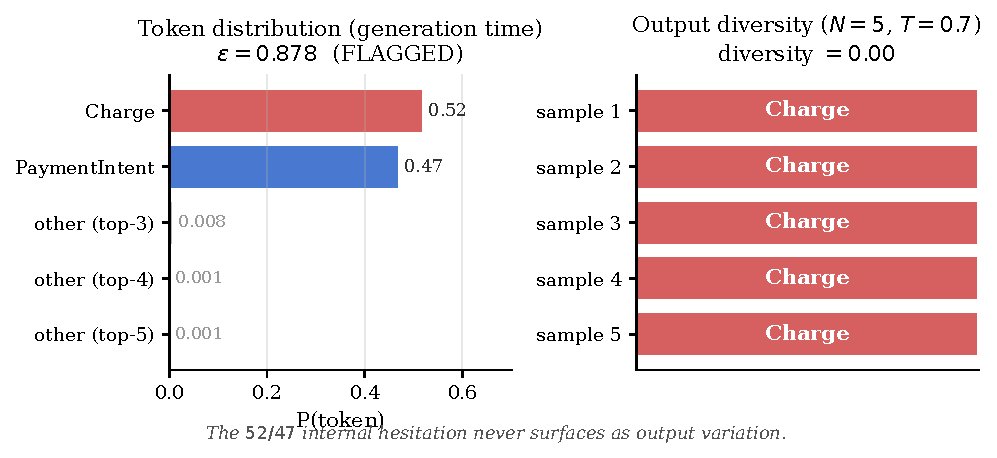
\includegraphics[width=0.85\textwidth]{figures/fig_intra_inter.pdf}
\caption{The intra/inter distinction made concrete on Stripe Scenario
A (GPT-4o). Left: the token distribution at the method-selector token
shows a near-tie ($P(\texttt{Charge}) = 0.52$, $P(\texttt{PaymentIntent})
= 0.47$), giving $\eps = 0.878$. Right: five independent samples at
$T=0.7$ all emit \texttt{Charge} (diversity $= 0.00$). Multi-sample
can only observe the right panel; the left panel is what \eps reads.
The $52/47$ internal hesitation never surfaces as output variation.}
\label{fig:intra-inter}
\end{figure}

Figure~\ref{fig:intra-inter} is the empirical proof of the intra/inter
distinction, not a theoretical assertion. GPT-4o with $\eps = 0.878$ on
Stripe chose \texttt{Charge} unanimously across all five samples. A
stronger multi-sample check would not recover the signal: there is no
output variation for a semantic-equivalence test or symbolic executor
to disagree about. Our multi-sample measurement is output-level (which
API was chosen); stronger equivalence checks~\cite{sharma2025multisample}
that compare code behaviour up to semantic equivalence would help on
Type 3 (implementation-approach) false positives, where two
semantically equivalent implementations are wrongly counted as
disagreement, but they cannot recover intra-generational API-choice
uncertainty that produces unanimous output.

UQLM~\cite{uqlm2024} is the closest published off-the-shelf tool in this
family; its \texttt{BlackBoxUQ} method samples each prompt 5 times and
scores semantic disagreement via a DeBERTa NLI model. On our benchmark
it detects $5\%$ of HIGH-risk prompts at $0\%$ LOW false-positive rate
--- a result driven by the same structural limit: the model is
behaviourally consistent even when internally uncertain, so NLI-based
clustering reports confidence $\approx 1.0$ on $29$ of $30$ prompts.

\subsection{Static analysis}
\label{subsec:static-cov}

Static analysis and linter rules catch \emph{known}-bad patterns for
libraries where deprecation has been encoded into a ruleset; \eps fires
where the model itself hesitated, including decisions not yet in any
ruleset (a library updated last week, a half-migrated codebase, an
internal rename). The two are complementary and address different
failure modes. Static analysis is the floor under \eps; \eps operates
in the gap where rules do not yet exist. Primary experiments use
OpenAI plus DeepSeek V3 via Together AI; Anthropic exposes logprobs via
streaming, and vLLM exposes the full top-$k$. The method requires only
top-$k$ logprobs --- no model-internal access.

\subsection{Summary}
\label{subsec:comp-summary}

\begin{figure}[H]
\centering
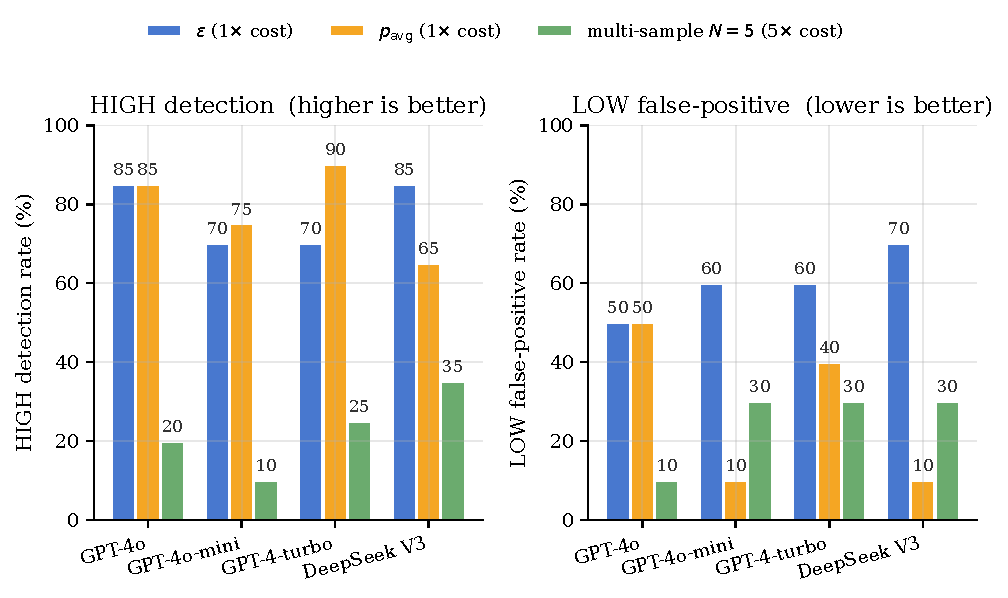
\includegraphics[width=\textwidth]{figures/fig_comparison.pdf}
\caption{Three-method comparison across four models. Left: HIGH
detection rate (higher is better). Right: LOW false-positive rate
(lower is better). \eps and \papg operate at $1\times$ API cost;
multi-sample at $N=5$ costs $5\times$. \papg is competitive with
\eps on raw detection but offers no token-level attribution;
multi-sample is structurally blind to intra-generational uncertainty.}
\label{fig:comparison}
\end{figure}

The empirical picture is honest. \papg matches or outperforms \eps on
raw detection for three of four models at the same API cost; its gap
with \eps is token-level localization, not raw rate. Multi-sample, at
$5\times$ the cost, reaches $10$--$35\%$ detection --- a structural
limit, not an implementation defect.
